\documentclass[12pt]{article}
\usepackage[a4paper, margin=1in]{geometry}
\usepackage{graphicx, microtype}
\usepackage{multicol,multirow}
\usepackage{natbib,tipa}

\title{Supplementary Information -- Morphological convergence as on-line lexical analogy}
\author{P\'eter R\'acz, Clay Beckner, Jen Hay, and Janet B.\ Pierrehumbert}

\usepackage{Sweave}
\begin{document}
\Sconcordance{concordance:si.tex:si.Rnw:%
1 9 1 1 0 2 1 1 58 26 1 1 10 35 1 1 48 6 1 1 2 16 0 1 3 35 1 1 20 24 1 %
1 87 1 2 19 0 1 3 32 1 1 31 8 1 1 27 1 1 1 2 19 0 1 3 31 1 1 21 1 51 1 %
3 20 0 1 2 6 1 1 36 6 1 1 21 6 1 1 40 1 3 14 0 1 2 1 3 14 0 1 2 17 1 1 %
14 30 1 1 24 1 4 15 0 2 3 15 0 1 2 8 1 1 50 2 1 1 17 1 2 15 0 1 2 6 1 1 %
80 1 1 2 2 14 1}



\maketitle

\noindent This is an Sweave file. The Rnw source file contains the code used to compile the pdf output file. It also contains additional code sections that help replicate the results. The files also contain pointers to further detail in the supplementary depository that accompanies the paper. 

\noindent In this supplementary information, we detail (\ref{appendixverbs}) the structure of our nonce verb stimuli, the setup of (\ref{appendixgcm}) the Generalized Context Model (GCM) and (\ref{appendixmgl}) the Minimal Generalization Learner (MGL), and (\ref{appendixgcmvsmgl}) how these models compare. 
We illustrate the models using fits on our \emph {baseline} data. 

We also discuss model selection in analysing our regression data (\ref{appendixregression}), how the two learning models compare on our baseline data (\ref{appendixgcmmglresidualization}), and how they compare on our ESP post-test data (\ref{mglgcmposttest}). 

Sections (\ref{appendixgcm}) and (\ref{appendixmgl}) also appear in the main text of  R\'acz et al. (2020), as Appendices A and B. However, this material is included here so that this Supplement can serve as a standalone document for readers who are interested in the technical details of our study. 

\section{Regular and irregular verbs in English \label{appendixverbs}}

Four irregular verb classes were defined for our stimuli, based on the vowel alternation and affixation processes that apply to the stem:

\begin{itemize}
    \item DROVE (\textipa{[aI]}/\textipa{[i]} $\rightarrow{}$ \textipa{[oU]})
    \item SANG (\textipa{[I]} $\rightarrow{}$ \textipa{[\ae]})
    \item KEPT (\textipa{[i]} $\rightarrow{}$ \textipa{[E]}Ct)
    \item BURNT (\textipa{[3]}/\textipa{[E]}/\textipa{[I]} $\rightarrow{}$ \textipa{[3]}/\textipa{[E]}/\textipa{[I]}Ct)
\end{itemize}

In the baseline experiment, participants are also tested on monosyllabic verbs that do not change in the irregular past tense (e.g.\ {\em cut}, {\em hit}). These forms are strong outliers and are not reported in the data.

The stimuli for the ESP experiment, 156 nonce verbs across four classes, are shown in Table 1 in the main text. Our formal criteria are based on the behavior of existing verbs in English and their categorization by \cite{bybee1982rules}, \cite{moder1992productivity}, and \cite{albright2003rules}. We made some adjustments to their categories. For instance, our DROVE class is a generalized version of Moder's class 4, described using the \textipa{[aI]}$\rightarrow{}$\textipa{[oU]} alternation but also including {\em weave}. (In contrast, Albright \& Hayes restrict this class to this alternation.) The verb classes could be defined in a number of ways and still be mostly consistent with the work of Moder, for instance. We have trialed a set of possible small changes and found that they have no major effect on our overall results.


\section{Implementation of the Generalized Context Model\label{appendixgcm}}

\subsection{Outline}

Our implementation of the GCM evaluates the competition between two categories, {\em regular} and {\em irregular}, for each nonce verb base form. The framework of \cite{nosofsky1990relations} is adapted to morphophonology by using a segmental similarity calculation based on natural classes \citep{frisch1997similarity}. The same treatment of segmental similarity is used in the implementations of the GCM in \cite{albright2003rules} and \cite{dawdy2014learnability}. We build on \cite{dawdy2014learnability} in that we define our categories based on formal similarity. 

\begin{quote}
 \texttt{The implementation of the GCM is laid out in models/gcm/gcm.html}.
\end{quote}

\subsection{Training data}

Participants are presented with a sequence of nonce verb base forms, and have to pick either a regular or an irregular past tense form for each. The irregular past tense form is pre-determined by the class for the stem, so that, for a given verb, the participants can only choose between the regular past tense form and the irregular past tense form we assigned to the verb. (So, for instance, for {\em splive}, a verb in the DROVE class, they can choose either {\em splived} or {\em splove}, but not {\em splift} or {\em sploven}, etc.) For a given class (such as DROVE verbs), the GCM has a choice between two sets of verb types. 

The irregular set consists of verb types in \textsc{Celex} that form their past tense according to the pattern captured by the class (such as an \{\textipa{[aI]},\textipa{[i]}\} $\rightarrow{}$ \textipa{[oU]} alternation). 
The regular set consists of verb types that have base forms that are similar to these irregular forms but have a regular {\em -ed} past tense form as well as miscellaneous regular verbs -- those that do not belong to our schemata . We narrow the regular set to monosyllabic forms. However, all polysyllabic irregular forms that could serve as a point of comparison are compounds based on monosyllabic forms (an example is {\em overwrite}, a compound form of irregular {\em write}). (A compound form might be more regular than a simplex form, but \textsc{Celex} will list both the regular and the irregular variant in both cases.) Table \ref{regexesforgcm} shows the descriptions of the verb classes using regular expressions. 

\begin{table}[ht]
\centering
\begin{tabular}{lllll}
\hline
& \multicolumn{2}{l}{input} & alternation \\
class & regular expression & IPA & \\
\hline
DROVE   & \texttt{[i2][zvdltnk]\$}  & $\{$\textipa{i},\textipa{aI}$\}$ + $\{$z,v,d,l,t,n,k$\}$ \#\# & $\{$\textipa{i},\textipa{aI}$\}$ $\rightarrow{}$ \textipa{oU}\\
SANG    & \texttt{I(m$|$N$|$Nk)\$}  & $\{$\textipa{I}$\}$ + $\{$m,\textipa{N},\textipa{Nk}$\}$ \#\# & \textipa{I} $\rightarrow{}$ \textipa{\ae} \\
KEPT    & \texttt{i[lpnm]\$}       & $\{$\textipa{i}$\}$ + $\{$l,p,n,m$\}$ \#\# & \textipa{i} $\rightarrow{}$ \textipa{E}Ct \\
BURNT   & \texttt{[3EI]nl\$}     & $\{$\textipa{3},\textipa{E},\textipa{I}$\}$ + $\{$n,l$\}$ \#\# & $\{$\textipa{3},\textipa{E},\textipa{I}$\}$ $\rightarrow{}$ $\{$\textipa{3},\textipa{E},\textipa{I}$\}$Ct \\

\hline
\end{tabular}
\caption{Descriptions of verb classes in the GCM. `C' marks any consonant.}
\label{regexesforgcm}
\end{table}


Our starting point for the training set, following \cite{albright2003rules}, is the list of verbs in the \textsc{Celex} corpus (\citealt{baayen1993celex}, based on \citealt{sinclair1987}) with a token frequency of 10 or above, encompassing 3156 forms. However, similarity requirements restrict the respective training sets. We use the {\em DISC} transcription in which each contrastive segment of English is represented by a unique character (\texttt{dr2v} equals \textipa{[draIv]}).

Table \ref{gcmsetsize} shows the number of verbs in \textsc{Celex} that were used as training sets for our verb classes. The irregular set consists of forms that match the schema and are irregular. The regular set contains schema matches which are regular, in addition to miscellaneous regulars. The miscellaneous set consists of monosyllabic verbs that do not belong to any of the schemata and are regular. These are included in the regular training set of \textsc{ each} verb class. 

The model calculates the similarity of a given nonce verb to the regular and the irregular set. Comparisons to stems in other classes are not calculated, as past tense markings for these classes were not available to participants in the forced-choice tasks.

% latex table generated in R 3.6.2 by xtable 1.8-4 package
% Thu Jan 30 09:32:35 2020
\begin{table}[ht]
\centering
\begin{tabular}{rllll}
  \hline
 & verb class & irregular set & regular set & miscellaneous regular verbs \\ 
  \hline
1 & BURNT & 6 & 42 & 1218 \\ 
  2 & DROVE & 14 & 83 & 1218 \\ 
  3 & KEPT & 12 & 31 & 1218 \\ 
  4 & SANG & 8 & 13 & 1218 \\ 
  5 & sum & 40 & 169 & 1218 \\ 
   \hline
\end{tabular}
\caption{Number of forms in each verb class, GCM training data} 
\label{gcmsetsize}
\end{table}
\subsection{Estimation}

To calculate the similarity between two words, we first compute their dissimilarity. This is achieved using the string-edit (Levenshtein) distance, which is the smallest number of changes needed to transform one word into the other. Costs range from 0 (the corresponding segments are identical) to 1 (inserting or deleting an entire segment). Following \cite{albright2003rules} and \cite{dawdy2014learnability}, costs between 0 and 1 are assigned to corresponding segments that are not identical, based on how much the segments differ. 

All parts of the word are weighted equally, because although there is evidence that past tense formation in English is predominantly driven by overlaps in word endings, onsets also play a role. (cf. the predominance of \emph {s}(+stop) onsets in irregular verbs forming the past tense with a vowel change, e.g.\ {\em stink}, {\em sink}, etc. -- see \citealt{bybee1983morphological}). 

The following transformation, originating with \cite{nosofsky1990relations}, is used to convert dissimilarity into similarity:

\vspace{1cm}
$\eta_{ij} = \exp {(- d_{ij} /s)^p}$
\vspace{1cm}

In the equation above, $\eta_{ij}$ represents the similarity between form $i$ and form $j$, while  $d_{ij}$ is the dissimilarity between the two forms. $s$ and $p$ are free parameters.  

We explored a range of parameter settings and use $s = 0.9$ and $p = 1$ which provide the best model fit on the baseline data. (In contrast, Albright and Hayes use $s = 0.4$ and $p = 1$.)

When {\em p} is set to 1, as here, the similarity function is an exponential, rather than a Gaussian, function of the dissimilarity. The weighting parameter {\em s} controls how quickly the similarity decreases as the difference (or distance) between the forms increases. When {\em s} is small, the behavior of the model will be dominated by the small group of instances that differ very little from any given novel form. As it becomes larger, instances that differ more increase their influence on the overall model behavior
 \citep{nosofsky1990relations,nakisa2001dual,albright2003rules,dawdy2014learnability}. Thus, {\em s} effectively controls the size of the set of verbs that will be taken into account in determining the support for the regular versus the irregular outcome.

The overall similarity $S_{iC_J}$ of a test form $i$ to a set
$C_J$ is calculated by summing the similarity $\eta_{ij}$ of each member $j$ of class $C_J$ to the test form $i$, and dividing by the summed similarity $\eta_{ij}$ of each member $k$ of class $C_K$ (the class of all stored forms) to the test form $i$. 
This calculation is summarized in the following equation.

\vspace{1cm}
$S_{iC_J} = \frac{{\sum_{j \in C_J } \eta_{ij} } }{{\sum_{k\in C_K } \eta_{ik} }}$
\vspace{1cm}

\subsection{Output format}

The overall score used in our analyses is the {\em regularity score}, which is the complement to the {\em irregularity score} and reaches a maximum of 1.0 when the output is most likely to be regular. Unlike \cite{dawdy2014learnability}, there is no decision rule on top of the scoring, such that any form that is more likely than not to be regular is predicted to surface as regular all the time. This specific decision rule is statistically optimal, and was imposed in \cite{dawdy2014learnability} in order to determine the ceiling performance for a computational model. The present paper, in contrast, analyzes data aggregated across human participants with differing decision thresholds. As discussed in \cite{schumacher2014reconciling} and \cite{schumacher2017prior}, the input-output relationship in such aggregated data are typically reported to be nearly probability-matching. 

We standardize the regularity score to match the range of participant responses: [0,1]. The modified score is interpretable as the probability that the outcome will be regular in aggregated data. It is also appropriate to attribute this type of gradience to people's initial expectations about other people's behavior, on the assumption that people realistically encode the variability they have encountered.

\subsection{Example: {\em splive}}


The nonce form {\em splive} belongs to the DROVE class in our model. The two past forms of {\em splive} in the experiment are regular {\em splived} and irregular {\em splove}. It is compared to 1301 regular verbs -- these are 83 verbs that match the DROVE schema (e.g.\ {\em side, hive, line}) and 1218 miscellaneous verbs. It is also compared to 14 irregular verbs (e.g.\ {\em drive, stride, smite}) in this class. Overall, it is more similar to the regular set: its {\em regularity score} is 0.57.   

\section{Implementation of the Minimal Generalization \\ Learner}\label{appendixmgl}

\subsection{Outline}

The Minimal Generalization Learner is an algorithm for forming input-output rules of varying generality, which then compete to generate the output. 

The Minimal Generalization Learner is implemented here from materials made available by Albright and Hayes \citep{albright2003rules}. These include their Segmental Similarity Calculator, implementing the natural class based similarity metric due to \cite{frisch1997similarity}, also used in the GCM implementation. Due to issues with the MGL code, we had to fit the MGL separately for participants.

\begin{quote}
 \texttt{The implementation of the MGL is laid out in models/mgl/mgl.html}.
\end{quote}

\subsection{Training data}

For our model fitted on our baseline nonce word stimuli, the MGL is trained on regular and irregular English verbs with a minimum frequency cutoff of 10 in \textsc{Celex} \citep{baayen1993celex}, encompassing 4160 past/present verb transcriptions. 

The MGL builds rules based on all verb forms in \textsc{Celex} with a token frequency of 10 or above. However the structural descriptions of the resulting rules do not cover all these forms. Table \ref{mglsetsize} shows the number of unique forms covered by the structural descriptions of the `regular' and `irregular' rules that are relevant to each class. 

The MGL generates multiple possible past tense forms for each nonce verb. We only consider those rules {\em relevant} that generate the past tense forms that appear in the experiment (e.g.\ {\em splive} : {\em splived} / {\em splove}). There is at most one relevant regular rule and one relevant irregular rule for one verb, but multiple rules can generate the (ir)regular forms for each verb class. We return to this in the next section.

Note that the sets of exceptions and related forms of each rule can overlap, both respectively and with each other. As a consequence, the MGL rules apply to fewer forms than apparent from the table: 456 (instead of 617) in total.


% latex table generated in R 3.6.2 by xtable 1.8-4 package
% Thu Jan 30 09:32:36 2020
\begin{table}[ht]
\centering
\begin{tabular}{rllrr}
  \hline
 & category & rule.type & related forms & exceptions \\ 
  \hline
1 & burnt & irregular &  24 &  41 \\ 
  2 & kept & irregular &  10 &   9 \\ 
  3 & sang & irregular &  11 &  77 \\ 
  4 & burnt & regular &  38 &  21 \\ 
  5 & drove & regular &  29 &  27 \\ 
  6 & kept & regular &  67 &  41 \\ 
  7 & sang & regular &  47 &  38 \\ 
   \hline
\end{tabular}
\caption{Number of forms in each verb class, MGL training data} 
\label{mglsetsize}
\end{table}
\subsection{Estimation}

The MGL begins by considering the relationship between each verb and its past tense as a `rule'. For each pair of verbs in the training data, it then attempts to create a more general rule. It does so by aligning the wordforms and analyzing shared phonetic features. For example,  merging the word-specific rules for {\em ring/rang} and for {\em stink/stank} yields a more general rule that expresses the information that they share: \textipa{[I]} $\rightarrow{}$\textipa{[\ae]} / [+coronal, - cont] \underline{\hspace{0.5cm}} \textipa{[N]}. Each rule inferred in this way is then further generalized on the basis of more comparisons; for instance, taking note of {\em swim/swam} expands the \textipa{[I]} $\rightarrow{}$\textipa{[\ae]} rule to specify that it occurs before all [+nasal] consonants. 

The structural description for each rule has a {\em scope}, which is the number of verbs conforming to the description, to which the rule might apply. The number of {\em hits} is the number of such verbs where the rule generates the correct output. In our example, {\em think} and {\em blink} fall in the scope of the rule, but they are not hits, because their past tenses display other patterns ({\em thought} and {\em blinked})
The {\it raw confidence} of the rule is the ratio of hits to scope: 

\vspace{1cm}
$\mbox{\it Raw confidence} = \frac{\mbox{\it  hits}} {\mbox{\it  scope}}$
\vspace{1cm}

The raw confidence is 1.0 if the rule applies to all forms that meet its structural description.  It is less than 1.0 if some forms meeting its structural description have past tenses other than that predicted by the structural change. Raw confidence values of 0 are not found, because a rule needs to apply to two or more examples to be posited in the first place.

The MGL raw confidence metric is adjusted on the basis of user-specified confidence limits, to generate an {\em adjusted confidence score} that takes into account the amount and distribution of available data. The MGL's lower limit affects how much confidence is assigned to rules that have a small number of instances; generalizations that are based on a smaller number of word types are penalized. The MGL's upper limit curtails the application of seemingly general rules which are in fact driven by a more specific rule \citep{albright2002modeling}. The MGL is implemented here with its default settings, with the exception of the algorithm's confidence limits. We implement the MGL with lower and upper confidence limits of 55\% and 95\%, respectively, since these values afford the best fit to English verb data in \cite{albright2003rules}.

Note that the MGL algorithm automatically groups together verbs on the basis of shared phonological properties; thus, verbs are most likely to form strong generalizations with other verbs that share the same onset or rhyme. Attempts to merge diverse wordforms under a single generalization would be more likely to incur penalties (i.e.\ exceptions). This feature of the MGL is important for comparing with the methods of the GCM. Both algorithms allow for category-specific similarities to play a role in rule formation.

\subsection{Output format}\label{mgloutput}

Recall that in both our baseline and ESP experiment the trial task is prompted by a stem and offers a choice between a regular form and a specific irregular form, presented orthographically. In order to model this choice, we take the MGL rule for the stem that outputs the regular form (the {\em relevant regular rule}) and the rule that outputs the specific irregular form (the {\em relevant irregular rule}). If several regular / irregular rules generate the same form, we take the one with the highest {\em adjusted confidence}, following \cite{albright2003rules}. We use these rules to calculate the form's {\em relative (adjusted) confidence}.

Out of 156 test verbs in the ESP post-test, the \textsc{Celex}-trained MGL generates a {\em relevant regular rule} for every verb. It does not generate a {\em relevant irregular rule} for 28 verbs. These are all nonce verbs in the \textsc{KEPT} category (see\ Section 4.1 in the main text). In this category, irregular forms are derived from the stem through a vowel change (e.g. {\em greel} $\rightarrow{}$ {\em grelt}). The verbs missing the relevant irregular rule all have bases ending in $<$m$>$, $<$n$>$, or $<$l$>$. This is because, in our implementation, there is an insufficient number of verb types in the training set to support these irregular rules. Decreasing the cutoff criterion for the model leads to the generation of more of the currently `missing' irregular rules, but the overall model fit becomes worse (cf.\ below). Therefore, we keep the cutoff criterion and assume that the adjusted confidence of the irregular rule for these 28 verbs is zero. We then take the relative confidence of the regular rule as compared to the regular {\em and} the irregular rule for each verb and took this as the adjusted regular confidence of the given verb. (If the irregular rule is missing, the value of this adjusted regular confidence is 1.) This is given by the following equation:

\vspace{1cm}
$\mbox{\it Relative (adjusted) confidence} = \frac{\mbox{\it  adjusted confidence of relevant regular rule}} {\mbox{\it  adj.\ conf.\ reg.\ rule } + \mbox{ \it adj.\ conf.\ relevant irreg.\ rule}}$
\vspace{1cm}

This relative adjusted confidence represents the MGL regularity score for an item, to be compared against the regularity score from the GCM (see Section \ref{appendixgcm}).  

\subsection{Example: {\em splive}}



The two past forms of {\em splive} in the experiment are regular {\em splived} and irregular {\em splove}. The {\em relevant regular rule} that generates the regular past tense is `$\emptyset{} \rightarrow{}$ \textipa{[d]} / \{\textipa{D}, \textipa{S}, \textipa{T}, \textipa{Z}, f, s, v, z\} \underline{\hspace{0.5cm}}'. The {\em structural description} indicates that this is a suffixation rule that can apply to forms that {\em end in an anterior fricative} (a natural class in our feature system).  The {\em raw confidence} of this rule is 0.98. This is because this rule applies to most forms in its scope (698/712). The {\em adjusted confidence} is very similar: 0.968. This is because this rule applies to a large number of forms overall. The {\em relevant irregular rule} that generates the irregular form is `\textipa{[aI]} $\rightarrow{}$ \textipa{[oU]} / \{\textipa{D}, \textipa{Z}, \textipa{dZ}, d, l, n, r, z\} \underline{\hspace{0.5cm}}v'. It applies to \textipa{[aI]} in the nucleus {\em preceded by voiced anterior consonant and followed by \textipa{[v]}}. In \textsc{Celex},the rule applies to three forms ({\em drive, strive, dive}) and fails to apply to five ({\em arrive, thrive, contrive, rive, connive}). Its {\em raw confidence} is 0.375. Its {\em adjusted confidence} is slightly lower (0.366). This is because it applies to a smaller number of forms overall. The {\em relative (adjusted) confidence} of the predicted regularity of {\em splive} is $0.98/(0.98+0.37)=0.73$. The respective rescaled value is 0.363.

\section{Further notes on the GCM and the MGL \label{appendixgcmvsmgl}}

The training set for the GCM is focused initially; it is grouped into four verb classes and based on formal similarity with base forms of existing irregular verbs playing a role within each class. This, in effect, assumes lexical gangs as a starting point \citep{alegre1999rule}. In contrast, the MGL starts establishing rules across all forms in the starting dictionary.

As we see, however, the MGL also focuses the training set. The structural descriptions of the forms only cover a fraction of all verbs in the starting dictionary, organized by shared groups of segments. While disjunction increases the power of a theory (increasing the set of acceptable classes), disjunct classes frequently serve as input for phonological processes \citep{mielke2008emergence} . In the MGL, the disjunction emerges despite the lack of an initial specification: while one rule accounts for the specific behavior of a given form, multiple rules cover a given class. The number of regular and irregular rules posited by the MGL for each verb class can be seen in Table \ref{mglruleses}. 



% latex table generated in R 3.6.2 by xtable 1.8-4 package
% Thu Jan 30 09:32:36 2020
\begin{table}[ht]
\centering
\begin{tabular}{rllrr}
  \hline
 & category & rule.type & related forms & exceptions \\ 
  \hline
1 & burnt & irregular &  24 &  41 \\ 
  2 & kept & irregular &  10 &   9 \\ 
  3 & sang & irregular &  11 &  77 \\ 
  4 & burnt & regular &  38 &  21 \\ 
  5 & drove & regular &  29 &  27 \\ 
  6 & kept & regular &  67 &  41 \\ 
  7 & sang & regular &  47 &  38 \\ 
   \hline
\end{tabular}
\caption{The number of unique rules posited by the MGL in each verb class} 
\label{mglruleses}
\end{table}
Table \ref{mglruleseskept} shows the list of (irregular and regular) rules for one of the classes, the KEPT class. We choose this class as it provides a good illustration of the estimation process. An MGL rule describes an $A \rightarrow{} B$ {\em alternation} in an $XAY$ {\em environment}. Since the KEPT rules are all suffixing, the following environment ($Y$) is empty. For the preceding environment ($X$), we give a list of segments that are matched by the structural description if it applies to four segments or fewer. Otherwise, we give a phonological description. So, for instance, the first rule turns \textipa{[il]} to \textipa{[Elt]} following any obstruent. Note that in some cases, the MGL generates multiple rules for the same alternation (such as \textipa{ip} $\rightarrow{}$ \textipa{Ept}). As discussed in Section \ref{mgloutput}, in such instances, we choose the candidate rule with the highest adjusted confidence in order to calculate the MGL regularity score. (Fricatives and nasal consonants constitute a natural class in the segmental feature system used by \citealt{albright2003rules}.) 

Inspection of the table shows that the MGL fails to generate some expected irregular rules; in the KEPT class, the MGL omits rules for any stems ending in \textipa{[in]} or \textipa{[im]}. Under the MGL, there is not enough lexical support for irregular rules of these types, and yet participants do irregularize nonce forms like {\em cheen} and {\em kleem}  in the forced choice task. In this respect, the variegated similarity of the non-natural GCM class (which can be used to categorize {\em cheen}) allows for a better approximation of participant behavior. Note also that in some cases, the MGL generates an overly-specific rule; the rule for stems ending in [il] applies only after obstruents, whereas participants also irregularize KEPT stems with a sonorant in the onset ({\em greel}/{\em grelt}).    

% directly piping in this table from R would be difficult, but it's lookupable
\begin{table}[ht]
\centering
\begin{tabular}{lll}
  \hline
alternation & preceding environment\\ 
  \hline
\textipa{il} $\rightarrow{}$ \textipa{Elt} & obstruent \\ 
\textipa{ip} $\rightarrow{}$ \textipa{Ept} & \{j, l, r, w\} \\ 
\textipa{ip} $\rightarrow{}$ \textipa{Ept} & dorsal consonant\\
\textipa{ip} $\rightarrow{}$ \textipa{Ept} & l \\ 
\textipa{ip} $\rightarrow{}$ \textipa{Ept} & any consonant \\
\textipa{il} $\rightarrow{}$ \textipa{Elt} & fricative or nasal consonant \\
$\emptyset{}$ $\rightarrow{}$ \textipa{d}    & alveolars \\ 
$\emptyset{}$ $\rightarrow{}$ \textipa{d}    & \{b, m\} \\ 
$\emptyset{}$ $\rightarrow{}$ \textipa{d}    & alveolar fricative or nasal consonant \\ 
$\emptyset{}$ $\rightarrow{}$ \textipa{d}    & \{b, m, p\} \\
   \hline
\end{tabular}
\caption{The unique rules posited for the KEPT class}
\label{mglruleseskept}
\end{table}

The rule structure of the MGL likely follows from its parameter settings, which were tuned to optimize its performance on our fairly irregular-looking nonce word stimuli. It requires further work to determine the extent to which the MGL fit on individuals would improve if the MGL parameters were customized for individual participants.\\

\section{Regression modeling procedures}\label{appendixregression}



% latex table generated in R 3.6.2 by xtable 1.8-4 package
% Thu Jan 30 09:32:36 2020
\begin{table}[ht]
\centering
\begin{tabular}{rrrrr}
  \hline
 & Estimate & Std. Error & z value & Pr($>$$|$z$|$) \\ 
  \hline
(Intercept) & -0.108 & 0.161 & -0.672 & 0.501 \\ 
  verb\_baseline\_average & 8.259 & 0.686 & 12.040 & 0.000 \\ 
  bot\_lexical\_typicalityrandom & 0.043 & 0.169 & 0.253 & 0.800 \\ 
  bot\_lexical\_typicalityreversed & 0.035 & 0.173 & 0.204 & 0.839 \\ 
  participant\_prereg\_average & 7.125 & 0.563 & 12.667 & 0.000 \\ 
  bot\_regularisation\_rate-40\% & -0.456 & 0.185 & -2.468 & 0.014 \\ 
  bot\_regularisation\_rate+40\% & 0.549 & 0.166 & 3.307 & 0.001 \\ 
  verb\_baseline\_average:bot\_lexical\_typicalityrandom & -2.402 & 0.927 & -2.591 & 0.010 \\ 
  verb\_baseline\_average:bot\_lexical\_typicalityreversed & -2.127 & 0.955 & -2.226 & 0.026 \\ 
   \hline
\end{tabular}
\caption{Experimental Data, Post-test Regression Model Summary. Model formula: post-test regular response ~ verb baseline mean x lexical typicality + participant pretest mean + regularization shift + (1 + verb.baseline.mean | participant) + (1 | verb)} 
\label{regressiontable1}
\end{table}
Our regression model selection in this article proceeded as follows. Except where stated otherwise, we fit logistic mixed-effects regression models, using R's lme4 package \citep{bateslme4}. Non-significant predictors are removed from our models, as determined by a series of comparisons of nested models, using likelihood ratio tests in R's anova function. However, our model tables (e.g., Tables 5 and 6 in the main text) include the significance levels generated by lme4 summaries.  

We investigate maximal random effects structures, allowing for random intercepts for participants and stimulus items (verbs), as well as random slopes for all within-unit factors. We compare nested random effects structures as above, and retain any random slopes and intercepts which are supported by likelihood ratio tests \citep{baayen2008mixed}.

In the model in Table 5 in the main text, repeated here as Table \ref{regressiontable1}, we elect to mean center continuous variables to counteract collinearity that becomes evident when including the interaction between and {\em lexical typicality} .  Although some debate exists regarding the practice of transforming variables \citep{belsley1991conditioning,echambadi2007mean}, centering variables is common practice to remove nonessential ill conditioning, that is, relationships that inevitably exist between main and product terms \citep{aiken1991multiple,jaccard2003interaction, jaeger2008categorical}. We note that if {\em verb baseline mean} is {\em not} centered, collinearity is high (VIF=15.79) in this model. A non-centered model also yields a significant main effect for {\em lexical typicality}, with increased post-test regularization in the random and reversed conditions. However, we elect to take a more conservative approach by not including a potentially spurious main effect. Note that other than this main effect difference, models with and without centering yield results that are qualitatively indistinguishable; all other main effects and interactions are present in either case. The collinearity for the centered model (Table 5 in the main text) is acceptable, with a maximum VIF score of 2.9.


Since it is unclear whether the absence of a difference between random and reversed conditions is due to a lack of data, we refit the model with the baseline average : typicality interaction on the random and reversed conditions only. Then we calculated the Bayes Factor of the null model (with no interaction) over the full model (with interaction) using Bayesian Information Criteria calculated by lme4. The result strongly supports the null model over the full model, indicating that the preference for the null model is {\em not} due to the lack of evidence to reject it.

\section{Fits of the two categorization models on the baseline data}\label{appendixgcmmglresidualization}

We fit the Celex-GCM and the Celex-MGL on the baseline data to see how well they predict regularisation responses by the baseline participants. The Celex-MGL outperforms the Celex-GCM, if slightly. Both models contribute independently to explaining variation in the data.


The concordance indices of the Celex-MGL (0.586) and the Celex-MGL (0.581) on the baseline data are similar, with some edge retained by the MGL, as in the case of \citep{albright2003rules}. Our concordance indices are calculated using the somers2 function in R's \texttt{Hmisc} package \citep{harrell2014hmisc}. 

Since the regularity scores of the GCM and the MGL for the nonce verbs are correlated  (r $=$ 0.478), we use residualization to see whether the two models make separate significant contributions to explaining variation in the baseline dataset (Section 6.3 in the main text.)

We fit two simple linear regression models; no random effects are explored in these models, since we are merely predicting algorithmic scores for each item. We rescale and center GCM and MGL scores for the model fits. 


% latex table generated in R 3.6.2 by xtable 1.8-4 package
% Thu Jan 30 09:32:37 2020
\begin{table}[ht]
\centering
\begin{tabular}{rrrrr}
  \hline
 & Estimate & Std. Error & z value & Pr($>$$|$z$|$) \\ 
  \hline
(Intercept) & -0.525 & 0.124 & -4.219 & 0.000 \\ 
  r\_baseline\_mgl\_features & 1.347 & 0.093 & 14.482 & 0.000 \\ 
  r\_baseline\_gcm\_features\_residual & 1.423 & 0.128 & 11.100 & 0.000 \\ 
   \hline
\end{tabular}
\caption{MGL scores and GCM residuals, baseline data} 
\label{resid1}
\end{table}
% latex table generated in R 3.6.2 by xtable 1.8-4 package
% Thu Jan 30 09:32:37 2020
\begin{table}[ht]
\centering
\begin{tabular}{rrrrr}
  \hline
 & Estimate & Std. Error & z value & Pr($>$$|$z$|$) \\ 
  \hline
(Intercept) & -1.225 & 0.160 & -7.682 & 0.000 \\ 
  r\_baseline\_gcm\_features & 2.391 & 0.149 & 16.063 & 0.000 \\ 
  r\_baseline\_mgl\_features\_residual & 1.008 & 0.090 & 11.154 & 0.000 \\ 
   \hline
\end{tabular}
\caption{GCM scores and MGL residuals, baseline data} 
\label{resid2}
\end{table}
Model 1 predicts the GCM scores from the MGL scores (M1: GCM regular score  $\sim$ MGL regular score). Model 2 predicts the MGL scores from the GCM scores (M2: MGL regular score  $\sim$ GCM regular score). In two additional models, we then use the residuals from each model (M1, M2) as an estimate of the variation present in one score that cannot be attributed to the other.  First, we use the residuals of Model 1 in another, mixed-effects logistic regression model along with the MGL scores to predict regular responses in the baseline task (M3: regular response  $\sim$ MGL score + GCM residual + (1 + MGL score + GCM residual$|$participant) + (1 $|$ verb)). We then residualize for the MGL. We use the residuals of Model 2 along with the GCM scores in a similar logistic regression model (M4: regular response  $\sim$ GCM score + MGL residual + (1 + GCM score + MGL residual $|$participant)). 

The model summaries can be seen in Table \ref{resid1} (M3) and Table \ref{resid2} (M4). The residuals remain significant predictors in both models. Note that while this paper reports values fit to the baseline experiment data, the same pattern of results also holds for models fit to the pre-test data.

Although residualization is sometimes critiqued when used as a stopgap for collinearity or sign changes in a regression model \citep{wurm2014residualizing}, these concerns do not apply in the present case.  We use residualization as a tool to test whether one metric contributes beyond what is covered by a different metric of the same attribute, as in 
\cite{baayen2006morphological}, and as also acknowledged in \cite{wurm2014residualizing}. 

\section{Model fits on the post-test data}\label{mglgcmposttest}

We fit the Celex-GCM,the Celex-MGL, as well as the Individual-GCM and the Individual-MGL on the post-test data. Recall that the Celex-based models were trained on verbs in Celex. The individual-based models were trained for each participant, on Celex verbs as well as the co-player's responses in the ESP test. They were tested on the post-test for each participant, individually.

In the paper, we list four techniques of evaluating model fit. We go through these in turn.

\subsection{Comparing concordance indices}

First, we calculated concordance indices for the Celex- and individual-models on the post-test data of the ESP experiment.


Table \ref{modellingsummary} summarizes the concordance indices between our data and the various categorization models. The \textsc{Celex}-MGL, outperforms the \textsc{Celex}-GCM on the post-test data to some extent, much like in the case of our baseline data. The individual-GCM considerably improves on the \textsc{Celex}-GCM in terms of explaining the post-test data. The individual-MGL also improves on the \textsc{Celex}-MGL, but to a lesser extent.

\begin{table}[h]

    \centering
    \begin{tabular}{lllll}
            & training data & method & test data & C\\
            \hline
\textsc{Celex}-GCM & real verbs & `analogy' & verbs in baseline &0.581\\
\textsc{Celex}-MGL & real verbs & `rules' & verbs in baseline &0.586\\ \hline
\textsc{Celex}-GCM & real verbs & `analogy' & verbs in post-test &0.602\\
individual-GCM & real verbs + verbs seen in ESP & `analogy' & verbs in post-test &0.681\\

\textsc{Celex}-MGL & real verbs & `rules' & verbs in post-test &0.61\\
individual-MGL & real verbs + verbs seen in ESP & `rules' & verbs in post-test &0.625\\
\hline
    \end{tabular}
    \caption{Summary of concordance indices between our data and the categorization models. The values above the line show the concordance indices for the baseline data, as reported in Section 6.3 of the main text. The values below the line show the indices for the ESP post-test data.}
    \label{modellingsummary}

\end{table}

The issue here is that a concordance index is not a statistical test, and does not provide a margin of error. The trends are apparent: the individual-GCM is more of an improvement than the individual-MGL. But the strength of these trends is less clear.

\subsection{Extra information provided by the individual model over the {\sc Celex}-model}

Second, we considered the amount of extra variation explained by the individual-model over the {\sc Celex}-model, for the MGL and the GCM, respectively.

Section 6.4 in the main text explains that we calculate the extra information given by the individual models by subtracting the {\sc Celex} model prediction from the individual model prediction for each item for each participant.


% latex table generated in R 3.6.2 by xtable 1.8-4 package
% Thu Jan 30 09:32:37 2020
\begin{table}[ht]
\centering
\begin{tabular}{rrrrr}
  \hline
 & Estimate & Std. Error & z value & Pr($>$$|$z$|$) \\ 
  \hline
(Intercept) & -2.951 & 0.295 & -10.007 & 0.000 \\ 
  r\_baseline\_gcm\_features & 4.369 & 0.425 & 10.284 & 0.000 \\ 
  gcm\_score\_diff & 2.612 & 0.470 & 5.563 & 0.000 \\ 
  participant\_prereg\_average & 5.289 & 0.602 & 8.788 & 0.000 \\ 
   \hline
\end{tabular}
\caption{Celex-GCM and individual score difference, post-test data} 
\label{indiv1}
\end{table}
% latex table generated in R 3.6.2 by xtable 1.8-4 package
% Thu Jan 30 09:32:37 2020
\begin{table}[ht]
\centering
\begin{tabular}{rrrrr}
  \hline
 & Estimate & Std. Error & z value & Pr($>$$|$z$|$) \\ 
  \hline
(Intercept) & -1.318 & 0.152 & -8.663 & 0.000 \\ 
  r\_baseline\_mgl\_features & 1.944 & 0.176 & 11.045 & 0.000 \\ 
  mgl\_score\_diff & 0.304 & 0.139 & 2.181 & 0.029 \\ 
  participant\_prereg\_average & 7.203 & 0.591 & 12.190 & 0.000 \\ 
   \hline
\end{tabular}
\caption{Celex-MGL and individual score difference, post-test data} 
\label{indiv2}
\end{table}
We do this for both the GCM  (Model 5: regular response  $\sim$ \textsc{Celex} GCM score + extra GCM information + participant pre-test mean + (1 + \textsc{Celex} GCM + extra GCM information$|$participant) + (1$|$verb) and the MGL (Model 6: regular response  $\sim$ \textsc{Celex} MGL score + extra MGL information + participant pre-test mean + (1 + \textsc{Celex} MGL + extra MGL information$|$participant)+ (1$|$verb)).

The extra information is a significant predictor of post-test responses in both models. However, this effect is much more robust for the GCM than for the MGL, as seen in Table \ref{indiv1} (M5) and Table \ref{indiv2} (M6). The individual-GCM has some success in modeling post-test behavior when trained with real English verbs and information from the ESP test, whereas adjustments made to the individual-MGL do not vastly improve predictive power. 

These techniques are indicative of the relative strengths of the individual-MGL and -GCM respective to their {\sc Celex}-counterparts and each other. However, they do not compare them directly. 

\subsection{Using combined model predictions to explain variation in participant post-test responses}


We used the {\sc Celex}-GCM, {\sc Celex}-MGL, individual-GCM, and individual-MGL together to predict participant post-test responses. The best model, reported in the paper, contains the {\sc Celex}-MGL and the individal-GCM. The summary can be seen in Table \ref{comp3}. 


% latex table generated in R 3.6.2 by xtable 1.8-4 package
% Thu Jan 30 09:32:38 2020
\begin{table}[ht]
\centering
\begin{tabular}{rrrrr}
  \hline
 & Estimate & Std. Error & z value & Pr($>$$|$z$|$) \\ 
  \hline
(Intercept) & -2.942 & 0.270 & -10.896 & 0.000 \\ 
  r\_baseline\_mgl\_features & 1.600 & 0.171 & 9.361 & 0.000 \\ 
  r\_individual\_gcm\_features & 2.786 & 0.378 & 7.369 & 0.000 \\ 
  participant\_prereg\_average & 5.437 & 0.585 & 9.298 & 0.000 \\ 
   \hline
\end{tabular}
\caption{Celex-MGL and Individual-GCM predict variation in the post-test} 
\label{comp3}
\end{table}
Goodness-of-fit tests show that model fit is significantly worse if we exclude {\sc Celex}-MGL ($\chi^2 = $ 201.86) or individual-GCM ($\chi^2 = $ 81.82) as predictors. It is not significantly better if we include individual-MGL ($\chi^2 = $ 0.09) or {\sc Celex}-GCM ($\chi^2 = $ 2.03).

\subsection{Visualising model contributions to explaining variation in post-test responses}

Figure \ref{bigfigure} shows how baseline and post-test regularisation means of words compare for participant responses, the GCM, and the MGL.


\begin{figure}
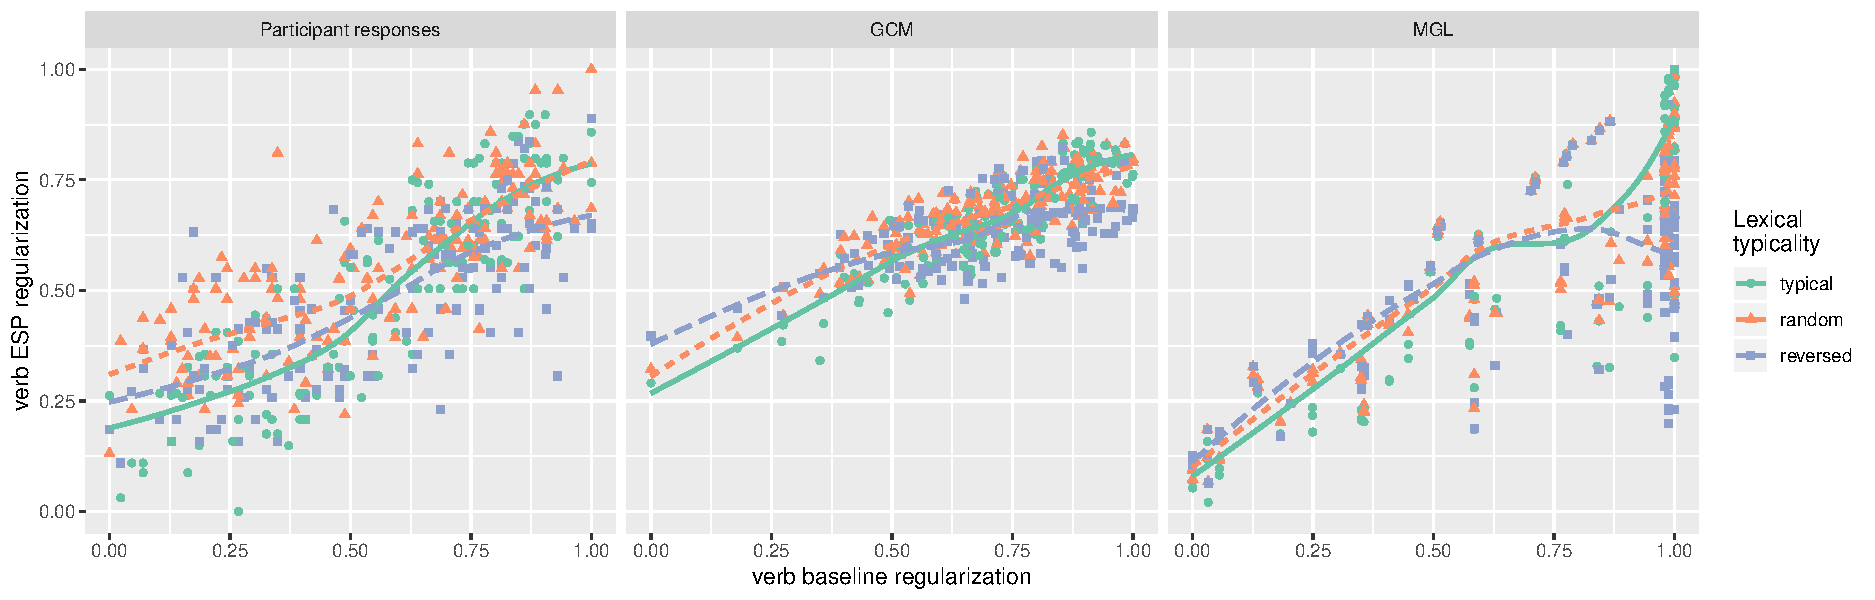
\includegraphics{si-model_figure2}
\caption{Baseline and individual regularisation weights: participants, GCM, MGL}
\label{bigfigure}
\end{figure}

The Figure shows the average baseline regularity (x axis) and the post-test regularity (y axis) of the verbs in the ESP experiment. The post-test values vary across the dimension of co-player lexical typicality. Loess smooths show the general trajectory of the effects of typicality. In the first panel, regularity translates to aggregate participant responses in the baseline and in the ESP post-test. In the second and third panels, regularity translates to regularity scores provided by the {\sc Celex}- and individual-GCM and -MGL. Values are rescaled for better comparison.

While the loess smooths are likely slightly overfit, they show the general trend in the raw data, which is echoed in the regression analysis in the main text: the "typical" trend of baseline-post-test difference is stronger than either the "random" or "reversed" trends. These are not very much different from each other. The differences are gradual. The GCM, while generally overestimating regularity, captures this gradual shift, since verb behaviour is shifted individually in the post-test. The MGL also overestimates regularisation. Since rules affect groups of verbs, rather than individual verbs, the post-test shifts are abrupt. The "typical" trend continues climbing after a longer plateau. However, the "random" and "reversed" trends trail off, where the "reversed" trend turns negative towards the higher tail of the distribution.


\newpage

\bibliographystyle{language}
\bibliography{racz_beckner_hay_pierrehumbert_2020}

\end{document}
